\documentclass{article}
\usepackage{amsmath, amssymb, xcolor, listings, booktabs, geometry}
\usepackage{graphicx}
\definecolor{codeblue}{RGB}{25,25,112}
\geometry{a4paper, margin=1in}

\begin{document}

	\section*{IMU Measurement Model with Sensor Offset and Misalignment}

	We consider an IMU mounted at a known offset $\mathbf{r}$ from the body reference frame origin, with a known fixed rotation $\mathbf{R}_{BS}$ from body frame ($B$) to sensor frame ($S$). The IMU provides measurements of linear acceleration and angular velocity. The 19-dimensional state vector is defined as:
	\[
	\mathbf{x} = \begin{bmatrix}
		\mathbf{p} \\
		\mathbf{q} \\
		\mathbf{v} \\
		\boldsymbol{\omega} \\
		\mathbf{a} \\
		\boldsymbol{\alpha}
	\end{bmatrix}
	=
	\begin{bmatrix}
		p_x, p_y, p_z \\
		q_0, q_1, q_2, q_3 \\
		v_x, v_y, v_z \\
		\omega_x, \omega_y, \omega_z \\
		a_x, a_y, a_z \\
		\alpha_x, \alpha_y, \alpha_z
	\end{bmatrix},
	\]
	where $\mathbf{q}$ is the quaternion representing orientation from inertial to body frame.

	\section*{IMU Measurement Model}

	\begin{figure}[h]
		\centering
		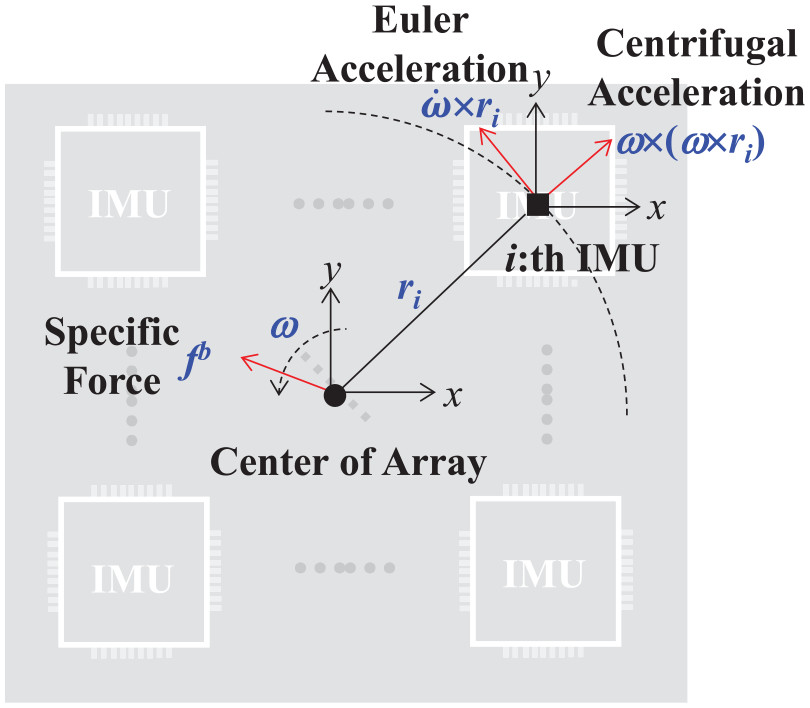
\includegraphics[width=0.8\textwidth]{imu_forces.jpeg}
		\caption{Illustration of IMU Forces and Motion Dynamics}
		\label{fig:imu_forces}
	\end{figure}
	The IMU provides two measurements:

	\begin{enumerate}
		\item Accelerometer measurement ($3\times1$):
		\[
		\mathbf{a}_{IMU} = \mathbf{R}_{BS}\left[\mathbf{a} + \mathbf{R(q)}^T \mathbf{g} + \boldsymbol{\alpha}\times \mathbf{r} + \boldsymbol{\omega}\times(\boldsymbol{\omega}\times \mathbf{r})\right]
		\]

		\item Gyroscope measurement ($3\times1$):
		\[
		\boldsymbol{\omega}_{IMU} = \mathbf{R}_{BS}\,\boldsymbol{\omega}
		\]
	\end{enumerate}

	Here:
	\begin{itemize}
		\item $\mathbf{R(q)}^T$ rotates vectors from inertial to body frame.
		\item $\mathbf{R}_{BS}$ is a constant rotation matrix from body to sensor frame (misalignment).
		\item $\mathbf{g}$ is gravitational acceleration in inertial coordinates.
		\item $\mathbf{r}$ is lever arm vector (body coordinates).
	\end{itemize}

	\section*{Bias Estimation with Sliding Window Averaging}
	Bias estimation is crucial for IMU accuracy, and the following sliding window method is employed:

	\paragraph{Bias Estimation Logic:} Given the current instantaneous bias estimates:
	\[
	\hat{\mathbf{b}}_{gyro} = \mathbf{gyro}_{measured} - \mathbf{gyro}_{predicted}
	\]
	\[
	\hat{\mathbf{b}}_{accel} = \mathbf{accel}_{measured} - \mathbf{accel}_{predicted}
	\]

	The updated biases are calculated using recursive averaging:
	\[
	\mathbf{b}_{gyro} = \mathbf{b}_{gyro} + \frac{\hat{\mathbf{b}}_{gyro} - \mathbf{b}_{gyro}}{N}
	\]
	\[
	\mathbf{b}_{accel} = \mathbf{b}_{accel} + \frac{\hat{\mathbf{b}}_{accel} - \mathbf{b}_{accel}}{N}
	\]

	Where $N$ is the sliding window size. This recursive averaging ensures gradual convergence to stable bias estimates by averaging recent observations.

	\section*{Stationary Detection Logic}
	Determining whether the IMU is stationary is essential for improving bias estimation reliability. The system is defined as stationary when the following three conditions are met:

	\begin{itemize}
		\item State velocities are sufficiently close to zero:
		\[
		||\mathbf{v}||^2 < \chi_{critical}^{6dof}
		\]

		\item State accelerations are sufficiently close to zero:
		\[
		||\mathbf{a}||^2 < \chi_{critical}^{6dof}
		\]

		\item The accelerometer norm is sufficiently close to the gravity constant within a defined confidence threshold:
		\[
		| ||\mathbf{a}_{measured}|| - g | < \chi_{critical}^{1dof}
		\]

	\end{itemize}

	If all three conditions hold true, the system is considered stationary, allowing for improved bias estimation and state initialization.
	\section*{Jacobian Derivation}
	The Jacobian matrix $\mathbf{H}$ is defined as:
	\[
	\mathbf{H} =
	\frac{\partial}{\partial \mathbf{x}}
	\begin{bmatrix}
		\mathbf{a}_{IMU}\\
		\boldsymbol{\omega}_{IMU}
	\end{bmatrix},
	\]
	thus it has dimensions $6\times19$.

	Each component of the Jacobian is derived stepwise as follows:

	\paragraph{Gyroscope Jacobian:} Since the gyroscope measurement is the body-frame angular velocity rotated into the sensor frame:
	\[
	\frac{\partial \mathbf{\omega}_{IMU}}{\partial \boldsymbol{\omega}} = \mathbf{R}_{BS}
	\]

	\paragraph{Accelerometer Jacobian:} The accelerometer Jacobian includes multiple components:

	- Linear acceleration mapping:
	\[
	\frac{\partial \mathbf{a}_{IMU}}{\partial \mathbf{a}} = \mathbf{R}_{BS}
	\]

	- Tangential acceleration term:
	\[
	\frac{\partial \mathbf{a}_{IMU}}{\partial \boldsymbol{\alpha}} = -\mathbf{R}_{BS} [\mathbf{r}]_\times
	\]

	- Angular velocity cross-product term: To differentiate $\mathbf{\omega} \times (\mathbf{\omega} \times \mathbf{r})$, we expand the cross product:
	\[
	\frac{\partial (\mathbf{\omega} \times (\mathbf{\omega} \times \mathbf{r})))}{\partial \mathbf{\omega}} = [\mathbf{\omega} \times \mathbf{r}]_\times - [\mathbf{r}]_\times [\mathbf{\omega}]_\times
	\]
	Thus,
	\[
	\frac{\partial \mathbf{a}_{IMU}}{\partial \boldsymbol{\omega}} = \mathbf{R}_{BS} \left([\mathbf{\omega} \times \mathbf{r}]_\times - [\mathbf{r}]_\times [\mathbf{\omega}]_\times\right)
	\]

	- Gravity Jacobian (quaternion effect on gravity rotation): For gravity vector $\mathbf{g}_W = [0, 0, g]^T$ in the world frame,
	\[
	\mathbf{g}_B = q^{-1} \mathbf{g}_W q = g \begin{bmatrix}
		2(q_xq_z - q_wq_y) \\
		2(q_yq_z + q_wq_x) \\
		1 - 2(q_x^2 + q_y^2)
	\end{bmatrix}
	\]
	The corresponding Jacobian is:
	\[
	\frac{\partial \mathbf{g}_B}{\partial \mathbf{q}} =
	\begin{bmatrix}
		-2gq_y & 2gq_z & -2gq_w & 2gq_x \\
		2gq_x & 2gq_w & 2gq_z & 2gq_y \\
		0 & -4gq_x & -4gq_y & 0
	\end{bmatrix}
	\]

	Finally, applying the sensor-to-body rotation for consistency:
	\[
	\frac{\partial \mathbf{a}_{IMU}}{\partial \mathbf{q}} = \mathbf{R}_{BS} \frac{\partial \mathbf{g}_B}{\partial \mathbf{q}}
	\]

	This expanded derivation ensures that all key contributors to IMU dynamics are captured in the Jacobian calculation.



	\section*{Conclusion}
	This enhanced IMU model integrates precise measurement prediction, robust stationary detection, and efficient sliding window bias estimation. The improved Jacobian derivation ensures accurate integration with state estimation frameworks. Together, these enhancements improve the system's stability, accuracy, and robustness in dynamic and stationary environments.
	\appendix

\appendix
\section*{Appendix: Important Considerations for IMU Model Testing}

Robust testing of the IMU model is critical to ensuring stable and accurate performance. The following considerations highlight key aspects to address when validating the IMU model:

\subsection*{1. Precision in Quaternion Handling}
\begin{itemize}
	\item \textbf{Quaternion Perturbations:} Since quaternions represent rotation, numerical drift can occur if precision is not carefully maintained.
	\item \textbf{Key Tests:}
	\begin{itemize}
		\item Use proper exponential map perturbations rather than naive additive perturbations.
		\item Verify that perturbations around each axis respect the expected behavior for both small and large angles.
	\end{itemize}
	\item \textbf{Pitfall to Avoid:} Directly modifying quaternion elements without re-normalization can introduce significant errors.
\end{itemize}

\subsection*{2. Jacobian Validation}
\begin{itemize}
	\item \textbf{Key Concept:} The Jacobian is crucial for linearization in estimation algorithms like Extended Kalman Filters (EKF). The Jacobian should match the actual behavior of the measurement model for small perturbations.
	\item \textbf{Key Tests:}
	\begin{itemize}
		\item Baseline Comparison: Validate that small perturbations produce measurement changes that closely match Jacobian-predicted deltas.
		\item Threshold Tuning: Select appropriate error thresholds — too tight can lead to false negatives; too loose can mask underlying problems.
	\end{itemize}
	\item \textbf{Pitfall to Avoid:} Using excessively large perturbations can break the linear approximation assumption that underpins Jacobian validity.
\end{itemize}

\subsection*{3. Angular Velocity and Acceleration Testing}
\begin{itemize}
	\item \textbf{Key Concept:} Angular velocity perturbations should match the rotational rate sensitivity defined in the model. The Coriolis term in the accelerometer model can amplify errors.
	\item \textbf{Key Tests:}
	\begin{itemize}
		\item Introduce small angular velocity perturbations and compare actual vs predicted changes in accelerometer outputs.
		\item Angular acceleration perturbations should similarly track predicted changes from the Jacobian.
	\end{itemize}
	\item \textbf{Pitfall to Avoid:} Neglecting Coriolis effects in validation can lead to false assumptions about model accuracy.
\end{itemize}

\subsection*{4. Gravity Alignment}
\begin{itemize}
	\item \textbf{Key Concept:} Gravity alignment is critical for orientation estimation in IMU models. Errors in quaternion logic or sign conventions can severely impact performance.
	\item \textbf{Key Tests:}
	\begin{itemize}
		\item Validate roll and pitch estimates by comparing against calculated angles:
		\[ \text{roll} = \arctan\left(\frac{a_y}{a_z}\right), \quad \text{pitch} = \arcsin\left(-\frac{a_x}{g}\right) \]
		\item Use gravity magnitude tests to confirm stability:
		\[ \| \mathbf{a}_{IMU} \| \approx 9.80665 \ \text{m/s}^2 \]
	\end{itemize}
	\item \textbf{Pitfall to Avoid:} Failing to differentiate between body-frame and world-frame gravity projections can lead to major orientation errors.
\end{itemize}

\subsection*{5. Sensor Misalignment}
\begin{itemize}
	\item \textbf{Key Concept:} The rotation matrix $\mathbf{R}_{BS}$ corrects for IMU mounting misalignment. Errors in this rotation matrix directly affect accuracy.
	\item \textbf{Key Tests:}
	\begin{itemize}
		\item Introduce intentional misalignment in test configurations and confirm correct compensation.
		\item Combine roll, pitch, and yaw misalignments to ensure robustness in all orientations.
	\end{itemize}
	\item \textbf{Pitfall to Avoid:} Assuming a perfect sensor-to-body alignment can hide real-world errors.
\end{itemize}

\subsection*{6. Bias Estimation}
\begin{itemize}
	\item \textbf{Key Concept:} Biases (especially for gyroscopes) drift over time. The recursive averaging method used in the code relies on stable stationary conditions for reliable bias estimation.
	\item \textbf{Key Tests:}
	\begin{itemize}
		\item Perform tests under both dynamic and stationary conditions to confirm that:
		\begin{itemize}
			\item Biases remain stable in stationary conditions.
			\item Bias estimation converges accurately under dynamic conditions.
		\end{itemize}
	\end{itemize}
	\item \textbf{Pitfall to Avoid:} Overestimating stationary conditions can cause biases to accumulate unnoticed.
\end{itemize}

\subsection*{7. Frame Conventions and Sign Ambiguities}
\begin{itemize}
	\item \textbf{Key Concept:} Quaternion conventions vary across libraries (e.g., Hamilton vs JPL convention). Additionally, gravity direction may be treated as either upward or downward in different implementations.
	\item \textbf{Key Tests:}
	\begin{itemize}
		\item Use practical IMU orientations (e.g., 20\textdegree roll, 30\textdegree pitch) to verify correct interpretation.
		\item Ensure yaw behavior is preserved when introducing combined pitch and roll rotations.
	\end{itemize}
	\item \textbf{Pitfall to Avoid:} Ignoring convention mismatches can produce inconsistent results across platforms.
\end{itemize}

\subsection*{8. Robustness to Numerical Noise}
\begin{itemize}
	\item \textbf{Key Concept:} IMU data often includes noise, especially in gyroscope and accelerometer readings. Tests should ensure that small noise fluctuations don't create disproportionate orientation drift.
	\item \textbf{Key Tests:}
	\begin{itemize}
		\item Introduce small Gaussian noise to simulated IMU measurements to assess filter stability.
		\item Validate that numerical instabilities don't propagate through Jacobian linearizations.
	\end{itemize}
	\item \textbf{Pitfall to Avoid:} Ignoring noise robustness can lead to performance degradation in real-world deployments.
\end{itemize}

\subsection*{Conclusion}
Effective IMU testing demands careful consideration of:
\begin{itemize}
	\item Numerical precision
	\item Jacobian accuracy
	\item Gravity alignment
	\item Sensor misalignment
	\item Bias estimation under realistic conditions
\end{itemize}
By designing rigorous tests that validate these aspects, you ensure the IMU model behaves reliably in both simulated and real-world conditions.



\end{document}
